\section{Design Landscape}
The purpose of designing a crypto-asset backed stablecoin is to create a stable asset out of a volatile asset. There are number of stablecoins using crypto-assets as collateral to issue stablecoins which shown a very broad design landscape for indirectly-backed stable coins.

In this part, we propose a systematical design decision model for indirectly-backed stablecoins. There are some key design decisions for each core feature. First we describe core feature and then key design decisions related to the main features and also we will discuss about pros and cons of each feature.

An overview of the indirectly-backed stablecoins design landscape is on Figure below:

\begin{figure*} [ht]
\centering
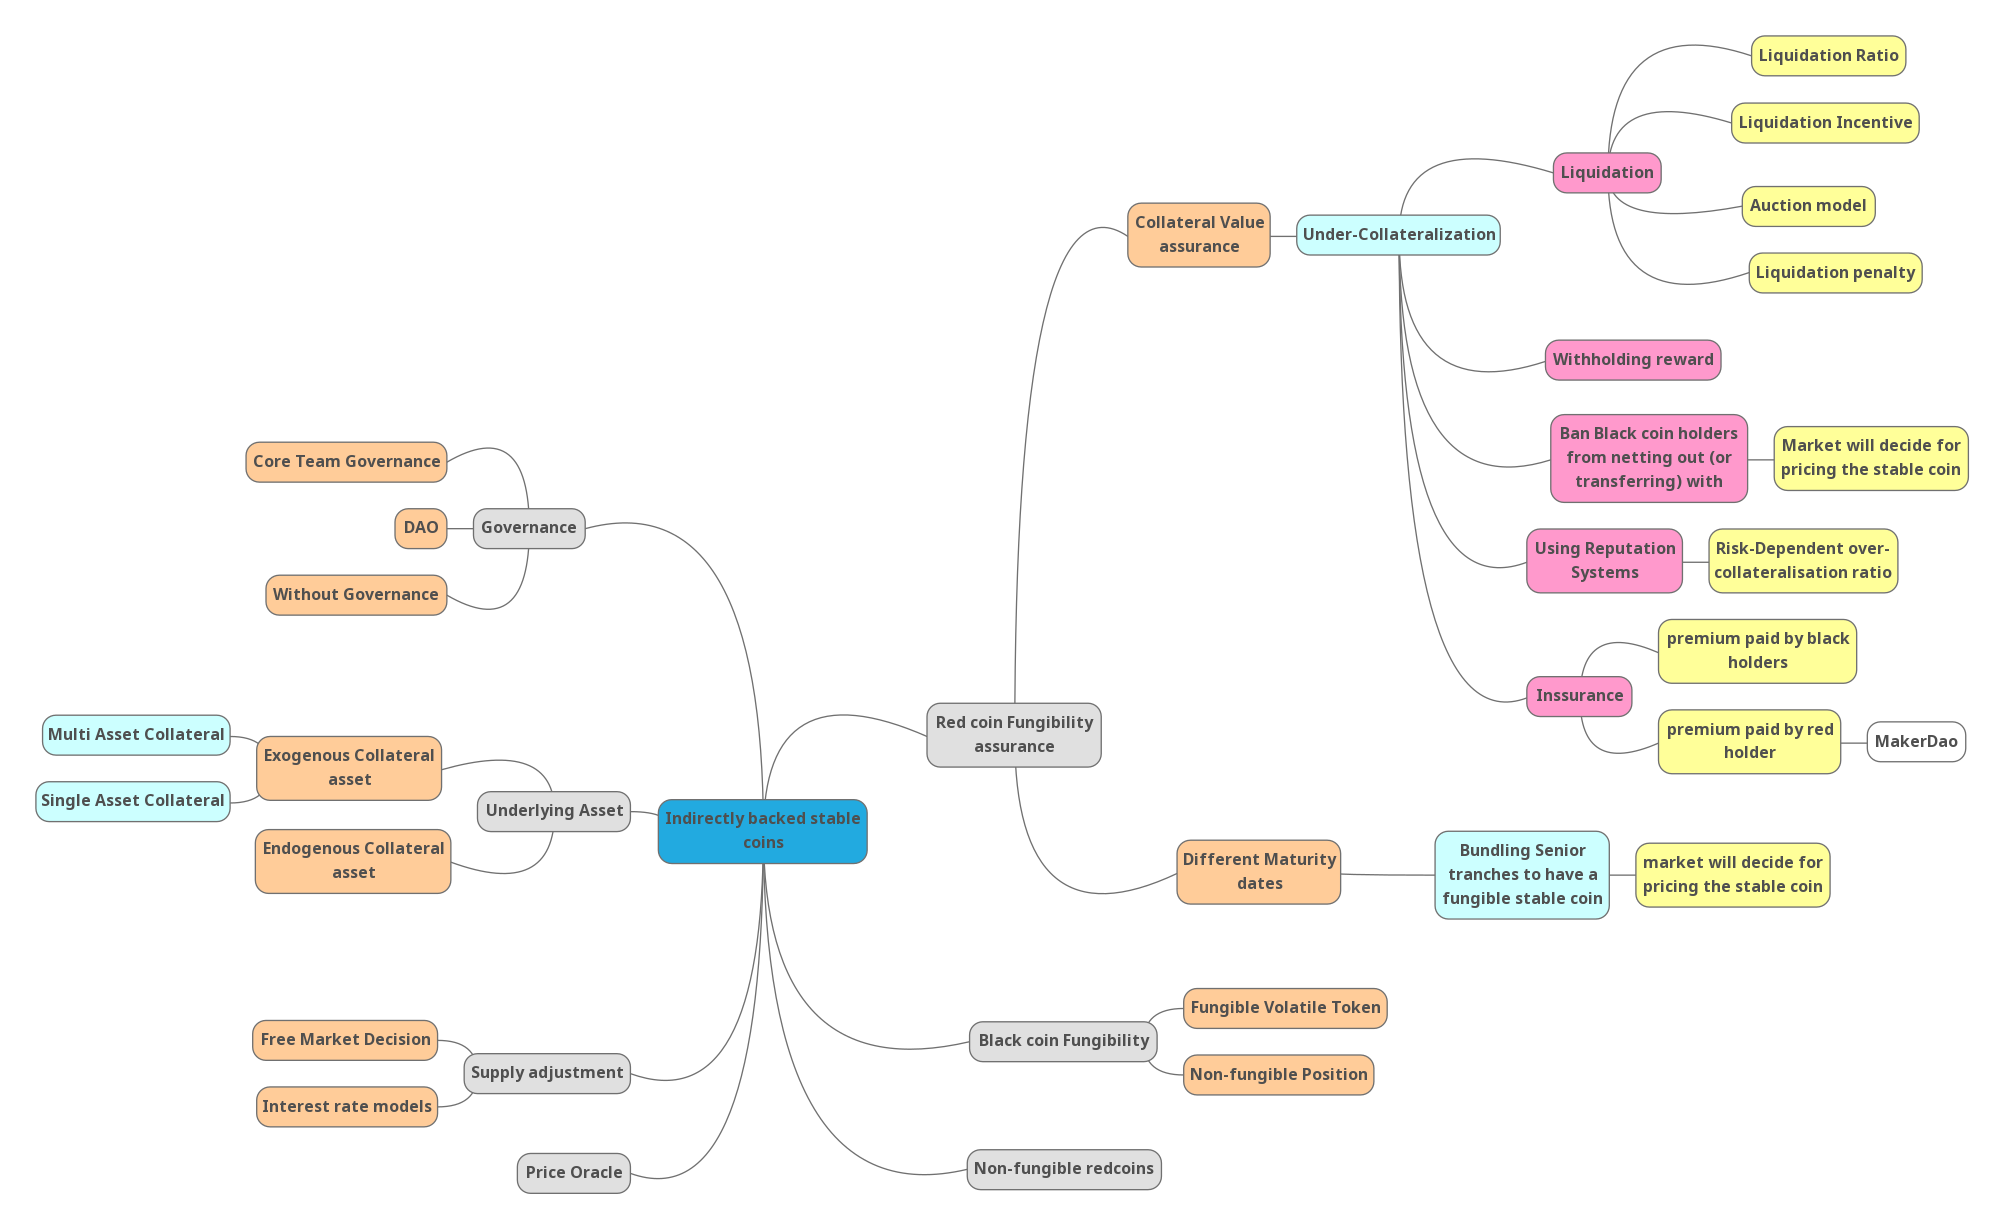
\includegraphics[width=16cm]{Mindmap}
\caption{overview of the indirectly-backed stablecoins design landscape}
\end{figure*}

\section{Fungibility}
Fungibility or Interchangeability refers to the ability of an asset to be exchanged by the same asset type with equal quality and quantity. For instance, dollar bills are fungible because people can exchange same amount of dollar without any frictions.

The first design decision is whether the tokens on the systems should be fungible or should be non-fungible. 

Fungiblity decision is devided into two parts:
\begin{itemize}
  \item Red coins Fungibility
  \item Black coins Fungibility
\end{itemize} 
We will discuss them seperately on next sections.


\subsection{Red coins Fungibility}
The Red coins, stable coin of the system, could be fungible or non-fungible. All existing indirectly-backed stablecoins are using fungible stablecoin design. However, it could be non-fungible as well.

\subsubsection{Non-fungible Red coins}
A stablecoin system designer could allow redcoins to be non-fungible. For instance, each token could be backed by different amount of ETHs without any limitation such as collateral ratio, liquidation and etc.

In this design class the Red coin and Black coin should be pair-wise. Because each pair-coin are backed by a different vault with specific amount of deposited ETH.

On order to specify each red coin there should be characterisitc to differentiate each red coin.

For example, each red coin could be marked with debt to collateral ratio, number of minted red coins divided by value of deposited ETH on the related vault, which clarify the safetiness of the redcoin.

So the buyer of redcoin could have an speculation on the price of each redcoin base on debt to collateral ratio.

However, there are reasons that push designers to make red coins fungible. The first reason is usability. Assume that Alice wants to buy 100 of redcoins. On the other side, Bob wants to sell just 30 coins, Carol wants to sell 50 and David wans to sell 20 red coins. Now Alice should make price assumption of three different coins and buy them with different prices which is not convenient for her.
The other issue with non-fungible red token is the price discovery. We need markets and crowd wisdom to offer different opinions of the value of an asset. The aggeregated results will discover the price of an asset. In non-fungible design there is not a straight relation between the price of each redcoin and the specific charectristic of them. So, Each person has a speculation for each coin. Because of non-fungibility the aggregations would not happened and so the real price will not be discovered.

The other reason is that stable coin users are willing to use the stable coins as a money. So, they need stable coins serve as a unit of account which means that you can price other goods or assets using the stable coin. In non-fungible design each red coin has a specific price. So, users can not price other goods based on the stable coin.

\textcolor{red}{Pros}:

\textcolor{red}{Cons}:


\subsection{Fungible Red coins}
As mentioned on the previos part, stable coin designers put all their effort to create a stable coin systems with fungible red coins. There are different mechanisms to bring fungibility into red coins. We categorize them into two key designs discussed on next sections.

\begin{itemize}
  \item Under-collaterallization
  \item Separate maturity dates
\end{itemize} 


\subsubsection{Collateral Value Assurance}

One of the ways to bring fungibility to red coins is to set a lower limit for vaults (Collateralization ratio). If the value of deposited ETH in a vault drops bellow a specific amount then the system decide to take some actions. This situation is called Under-collateralization.

Because all red tokens have high probability to be backed by at least collateralization ratio amount of ETHs it somehow secured the fungibility of redcoins.
 
In fact, all redcoin holders are sure that their red coins are backed by at least a dollar (with high probability) and there is no difference between their red coin and red coin of other people in this case.

There exist different designs to secure the vaults from under-collateralization scenario which is discussed in detail on next sections. Some of them are incentivizing vaults that keep their deposit more than collateralization ratio and some of them are disincetivazing the bad actors.

 
\paragraph{Liquidation}
This type of design is similar to the account margin in traditional finance. If the price of underlying asset drops and the value of the vault goes under collareralization ratio, the system will liquidate the vault.

Liquidation happens when it is probable that a vault is not able to pay its obligation and the vault's deposit will transfer to a person who take the responsibility of the debt of the vault. In other words, the liquidator should pay the borrowed redcoin (and other obligation in some designs such as staibility fee in MakerDAO) and receive the vault in exchange.

The majority of vaults are over-collateralized by liquidating under-collateralized vaults and if a vaults goes under-collateralized it will be liquidated. So, the redcoin holders are pretty sure that their coin is backed by at least over-collateralization amount of underlying asset and they can exchange their redcoins because the coins are similar and there is no difference between them.

Smart contracts are not able to trigger themselves. So, there should be an outsider player (like Keepers in MakerDao) to liquidate the alerted vaults. They should track the system and to find an under-collateralized vault and call liquidation function. Then the keeper will send the debt of the vault to the smart contract and receive the deposit on the vault in exchange.

There are design parameters in liquidation mechanism:

\begin{enumerate}
  \item Collateralization Ratio:
  This number shows the factor of over-collateralization. In fact the ratio between the value of the collateral on each vault and the value of borrowed redcoins should always be more than the collateralization ratio.
  
The collateralization ratio is depending on the volatility of the underlying asset. For instance, in MakerDAO platform the collateralization ratio for ETH vaults is 1.5. However, in Synthetix project it is 7.5 for SNX token which is more volatile than ETH.
  \item Liquidation Incentive:
A smart contract is not able to trigger itself. An outsider player named liquidator should pay the transaction fee to call the liquidation function of the smart contract. There are effective factors on the costs and profit of liquidators:
\begin{enumerate}
	\item Transaction fee:
	The liquidator should trigger the liquidation function, send the sufficient redcoins and play on the auction to win the vault and must pay transaction fees for these processes.
	\item Cost of capital: The liquidator has to pay the obligation in Redcoin to recieve the deposited coins on the vault. So the liquidator need enough liquidity for liquidation processes. There is an opportunity cost for the liquidator for not lending her capital and gaining interest out of it. On other scenarios the liquidator may just borrow the fund from lending platforms just to liquidate the vault and pay back the loan afterwards. There is a cost of borrowing in this scenario as well.So, there is a cost of capital for the liquidator.
	\item Price Feed: RB coin systems need the price of the underlying asset collected by oracles. Price inefficiency may impose extra costs to the liquidator
\end{enumerate}  

The designer has to incentivize the liquidators to watch the blockchain, find alerted positions, and then send transactions and liquidate them. 

The mechanism of the incentivization is different between protocols. A majority of platforms gives the liquidator discounts on the vaults. For instance in SAI (Single Collateral DAI) there was a \%3 discount on liquidation process. Other platforms are using auction models and let the market deciede about the value of the vault. 
  
  \item Auction model:
In case of liquidations different liquidators come up with an alerted position and want to liquidate it. The system designer have options for the decision of choosing the winner liquidator. 
The easiest implementation mechanism is the First Come First Serve However, it may not be fair to vault holder if the liquidator bids with low amount of redcoins. 

There are other auction-based mechanisms to find the liquidator. The question raised here is which type of auction is the most efficient and fair one for both bidders and vault holder.

MakerDao uses a combination of an absolute auction and a reverse auction model for the liquidation process.
The absolute auction is used till the bids cover the debt of the vault. After exceeding bids from the debt the auction will be reversed and the bidders bid on lower amount of the underlying assets in the liquidated vault for determined amount of DAI tokens that are specified on the privious auction step.
  
  \item Liquidation penalty:
Liquidation penalty is an extera punishment for the black coin holders to care about their debt to collateral ratio.
MakerDAO platform charges liquidated vault extera \%13 as a punishment for their vault holders. There are two main reason to add Liquidation penalty to the design:

\begin{enumerate}

  \item To force vault keepers to be over-collateralized
  \item To mitigate grinding attacks: grinding attack happens when the position holder intentionally unsafe its own position and participate in the liquidation auction against its own position to buy the liquidated asset cheaper.

\end{enumerate}
\end{enumerate}

\paragraph{Withholding rewards}

In the other types of the design such as liquidation, bad actors are disincentivized. But there is another approach to encourage users to act in a proper way, Incentivizing good actors.

For instance, in the Synthetix project users must collateralize SNX token (Synthetix network token) to receive sUSD (Synthetix stable coin pegging a dollar). There is no margin call or liquidation on the design. But there is a reward on the system for users who have more than the over-collateralization ratio on their vaults. 
In fact the Synthetix system has \%2 annual inflation on SNX token. The inflationary tokens are allocated to the vaults that have deposits more than collateralization ratio.
There is another reward source as well. The traders on Synthetix exchange pay transfer fees that are collected and distributed to the vaults holding more than collateral ratio.

The system incentivizes people to stake their SNX token and be over-collateralized to receive the rewards and there is no punishment in the system for bad actors.

\paragraph{Banning Black coin holders}

In the design of indirectly-backed stable coins the Red coins are not redeemable. In other words, The red coin holders are not able to give back their red coins and recieve the backed ETH directly. The only way to redeem redcoins is to have (or buy if possible) a black coin and request for netting out. 

In liquidation scenario, the designer is forced all black coin holder to be over-collateralized using liquidation punishment. Red coin holders and arbitragers are certain that with high probability each redcoin is backed by sufficient amount of ETH to be \$1 and there is no difference between redcoins which means redcoins are fungible.

In another scenario, the designer could remove liquidation and just ban black coin position holders from netting out. In fungible black coin holder design the designer ban black coin holders from transfering their token as well. 

The incentive for black coin holders to be over-collateralized has been reduced compare to liquidation design. But there is a huge incentive left for them to be over-collateralized. If the price of underlying asset drops the black coin holders are maybe want to sell their deposited asset. In this scenario just black coin holder that have over-collateralized vaults are able to net out and recieve their underlying asset and then sell it to the market.

This type of design will increase the fluctuation of redcoin price. The market will watch the aggregated collaterals on the system and the number of redcoins issued by the system and the price of underlying asset to evaluate the price of redcoins. So when the price of underlying asset drops the price of redcoins will reduce regarding to the underlying asset price. 

In this scenario redcoin holders are taking part of risk of underlying asset volatility risk.

\paragraph{Reputation systems}

In traditional finance, reputation systems and reputation scoring is used to remove or reduce the collateral needed for a specific financial transaction. In fact, parties are using their reputation as a collateral or source of trust for financial services. 

For example, in the FICO credit score system, users are able to enhance their credit limit by increasing their credit score. There is always a default risk on credits but the person who defaulted will be punished by credit score reduction. The bad actor will lose reputation score and forbiden from using plenty of financial services. Therefore, Users have enough incentive to pay their invoices.

A revoloution of decentralizing finance on top of blockchain technologies and cryptocurrencies began from early 2018 named Decentralized Finance (DeFi) movement. There are a myraid of different decentralized financial services out there such as MakerDAO, Compound, Synthetix, Aave and etc. 

There is not any difference between users that act properly on DeFi platforms and the bad actors. Obviously the DeFi ecosystem suffers from lack of a reputation system or reputation scoring. Using reputation system will incentivize users to act properly and reduce the default risk of the system. On the other side of the coin, the users with good reputation scores have new opportonities and the cost of defaulting will be increased for them.

There are hurdles for implementing an effective reputation systems on blockchains. Lack of strong identities and anonymity is one of them. Another restriction is users are able to create fake histories, However these are not impossible to address.

In case that our system concludes a trustworthy reputation system the designer is able to use reputation as a collateral. For instance we describe two different designs using reputation systems:
\begin{enumerate}
	\item Reputation-based collateral ratio: 
	In design of the system the collateral ratio could be dependent on the reputation of the user. In other words, the collateral ratio is higher for new users (users with no reputation) and lower for users that act properly for a long time.
	\item Reputation-based staibility fee
In systems like MakerDAO the DAI borrowers are obliged to pay a fee on their borrowing named staibility fee. This staibility fee is being set by Maker token holders.
	In a design based on reputation the staibility fee could be dependent on the reputation of the user. The reputable user is paying lower staibility fee compared to the new users.
\end{enumerate}
 
\paragraph{Insurance}

Insurance is used to hedge the risk of unexpected events in different systems. Under-collateralization of a vault is somehow an unexpected event on the RBcoin system. The designer could use insurance model to protect parties from financial loss in the case of under-collateralization. 

On insurance model the insurer will pay a premium to the insurance company and the company will protect the client from financial loss. 

In RBcoins there could be a built-in or outsourced insurance model to protect parties from undercollateralization loss. The question raised here is who should pay the premium?

\begin{enumerate}
	\item Premium pay by Red coin holders:
	It is very similar to Credit Default Swaps (CDS) on traditional finance. In this design the approach is that the red coin holders are lending some amount of money to black coin holders and black coin holders are borrowing from red coin holders to have a leveraged position on the underlying asset. In this situation the redcoin holders could pay insurance premium to the contract to protect themselves from default risk of black coin holders. In case of under-collateralization if the black coin holder could not afford the loss the insurance contract will pay the loss to the redcoin holder.

This type of design is implemented on MakerDAO platform in some ways. The DAI borrowers are paying a premium so called staibility fee to the system. These fees are collected on a pool named Maker Buffer pool. In the case of liquidation of a CDP, if the winner of the auction pays lower amount of the obligation of the vault the difference between the obligation and the paid amount will be paid by Maker Buffer pool.

	\item Premium pay by Black coin holders
In this type of design the black coin holders are paying the insurance premium. It is similar to the regular insurance contracts. For example, a person bought a house and insure it. Here the black coin holders are buying a position and pay the isurance premium. If the price of underlying asset drops and the vault going to be liquidated the insurance contract will pay on behalf of the insurer.
	\item Premium pay by both
	
In this scenario both Red and Black coin holders are paying the insurance premium to insure their positions. 
\end{enumerate}

\subsubsection{Different Maturity Dates}
In this type of design there are contracts like futures contract on Centralized finance (CeFi) which has a specific maturity date (M) and a strike price (K). strike price is the dollar value of ETHs that the parties agree that the stable player will recieve at the maturity date. 


A party who longs ETH and another party who bets on stability are collecting an amount of ETH (Q) and create new contract by tranching ETH into two different tokens. The stable token and a volatile token. Tranching in CeFi means when a highly volatile asset are spliting into different securities takes different risks. The junior tranche (volatile tokens) takes the majority volatility risk of the underlying asset and the senior tranche (stable coin) takes lesser risk. There is a maturity date for new contracts and each stable and volatile token depends on the day of the agreement. 


The stable tokens here are not fungible because each of them has a maturity date and the amount of underlying assets are varying day by day. To create a fungible coins, the stable tokens with different maturities are bundle together to create the Red coin which is stable coin of the system. The amount of redcoins the user get depends on the maturity date and the target price of the agreement.

For example, in Lien project the agreement between parties is at the maturity day the stable token holder will receive k USD if the deposited ETH worth k USD and the surplus will go to the volatile token holder. If the value of deposited ETH dropped below k USD then the stable token worth under k USD and the volatile token worth nothing. There are different specified maturity dates every 2 weeks. When a party receives the stable token, she will deposit it on a smart contract named iDOL to receive the stable coin (iDOL token). In fact, the iDOL contract bundles stable tokens with different maturities and strike prices and issue a stable coin out of this basket.

\textcolor{red}{Here I can describe Lien in details ...}:


\subsection{Black coins Fungibility}

The Black coins, volatile coin of the system, could be fungible or non-fungible. 

\subsubsection{Non-fungible Black coin}

In the majority of implemented indirectly-backed stable coin systems such as DAI, sUSD, USDx and etc. black coins are non-fungible. The vaults in these projects are holding different amounts of ETH coins, So the vaults are not fungible. 

Non-fungibility of black coins is one of the most important issues of the currently implemented projects. These systems are designed to attract users who need stability in addition to features of a cryptocurrencies. However, If Alice decides to issue new stable tokens, first she must create a pair of red coin and black coin. And she must hold the black coin because black coins are not transferable. So the users that need staibility should wait till another person who is willing to open a leveraged position create a new vault and want to sell her redcoins to the public.

The other problem of this type of design is the control of the demand and supply of the stable red coins. If the demand for redcoins suddenly increases in markets, the price of red coins on all markets will be increased. This is an opportunity to arbitragers to make a profit because the price of red coins are pegging a dollar. The arbitrager should issue new red token that costs \$1 for them and sell the red coins to the market and make profit. But the problem raised here, because if the arbitrager create a new vault then she should hold a non-fungible black token as well.So the arbitrager are able to stabilize the price just if the price in a few markets increased and on the others the price is \$1.

MakerDAO platform designers are using interest rate models to control the supply and demand of redcoins and black coins. This core design feature will be explained on the datail in next secttions.

\subsubsection{Fungible Black coin}

In case of fungible black coins the mentioned problem will be solved. If Alice wants a redcoin she could issue a new red, black coins pair and then sell her black coin in an exchange and use or keep her redcoin.

In my opinion it will boost the marketcap of indirectly-backed stable coins because people who are willing to use stable coins can issue them without any friction.

In this type of design there is no need to adjust interest rates to control the demand and supply of red coins. Because, if the price of recoins increases in a market the arbitragers are able to create new vaults, issue red and black tokens, sell the black coin on the markets and sell the newly generated redcoin which is worth a dollar to a person who is buying them more than a dollar. The arbitrager also could do all of these actions in a just one transaction using meta transaction method.

The problem of this type of desing is when the demand of redcoins are increasing and there is no demand for black coins. So, the arbitrager should sell the newly generated black coin lower than the issued price.

However it uses free market decisions to calculate the price of red and black coins which means if the price of red coin increases and there is no demand for black coins the price of redcoins will exceeds a dollar. 

The other problem of this type of design is the transaction fee for arbotragers. Because the arbitragers are using meta transactions they should pay high transaction fees for the arbitrage and it is not profitable in such cases.
